\documentclass[12pt]{article}
\usepackage{amsmath,amssymb}
%\usepackage{graphicx,psfrag,epsf}
\usepackage{graphicx}
\usepackage{enumerate}
\usepackage{natbib}
\usepackage{url} % not crucial - just used below for the URL
\setlength{\textheight}{9in}
\usepackage{longtable,booktabs}
\usepackage[unicode=true]{hyperref}
\providecommand{\tightlist}{%
  \setlength{\itemsep}{0pt}\setlength{\parskip}{0pt}}

\usepackage{tikz,  amsthm, multirow, float}
%\usepackage{tikz-3dplot}
\usetikzlibrary{arrows, shapes, positioning}
\usepackage{bm}

\usepackage{color}
\newcommand{\red}[1]{{\color{red} #1}}
\newcommand{\blue}[1]{{\color{blue} #1}}
%%INCLUDED-AK
\usepackage{amsthm}
\newtheorem{theorem}{Theorem}
\newtheorem{proposition}{Proposition}
\newtheorem{lemma}{Lemma}

\theoremstyle{definition}
\newtheorem{definition}{Definition}
\newtheorem{assumption}{Assumption}
\newtheorem{remark}{Remark}

\DeclareMathOperator*{\argmin}{arg\,min}
\DeclareMathOperator*{\argmax}{arg\,max}

\newcommand{\REP}{\mathrm{LREP}}
\newcommand{\DN}{\Delta_N}

\newcommand{\ma}{\mathrm{max}_{\boldsymbol \theta_N}}
\newcommand{\mi}{\mathrm{min}_{\boldsymbol \theta_N}}


\newcommand{\maa}{\mathrm{max}_{-\boldsymbol \theta_N}}
\newcommand{\mii}{\mathrm{min}_{-\boldsymbol \theta_N}}


\newcommand{\nv}{{n_{\scriptscriptstyle V}}}
\newcommand{\nh}{{n_{\scriptscriptstyle H}}}
\newcommand{\E}{E}

\newcommand{\elt}{A_{N}(\boldsymbol \theta_N) }
\newcommand{\Gam}{B_{N}(\boldsymbol \theta_N) }

\newcommand{\Gamc}{C_{N}(\boldsymbol \theta_N) }
\newcommand{\Gamt}{\Gamma_{N,2}(\boldsymbol \theta_N) }
%\pdfminorversion=4
% NOTE: To produce blinded version, replace "0" with "1" below.
\newcommand{\blind}{0}

% DON'T change margins - should be 1 inch all around.
\addtolength{\oddsidemargin}{-.5in}%
\addtolength{\evensidemargin}{-.5in}%
\addtolength{\textwidth}{1in}%
\addtolength{\textheight}{-.3in}%
\addtolength{\topmargin}{-.8in}%


\newenvironment{mybibliography}
[1]{\section*{References\markboth
 {REFERENCES}{REFERENCES}}
 \addvspace{6pt}
  \list{}{\labelwidth0pt
    \leftmargin40pt
    \itemindent-40pt
    \itemsep=0pt plus 1pt\parsep=0pt
    \usecounter{enumiv}%
  %  \let\p@enumiv\@empty
    \def\theenumiv{\arabic{enumiv}}}%
    \def\newblock{\hskip .11em plus.33em minus.07em}%
    \sloppy\clubpenalty4000\widowpenalty4000
    \sfcode`\.=1000\relax}


\let\BeginKnitrBlock\begin \let\EndKnitrBlock\end
\begin{document}


\def\spacingset#1{\renewcommand{\baselinestretch}%
{#1}\small\normalsize} \spacingset{1}

\title{\bf SUPPLEMENTARY MATERIAL TO:\\
Simulating Markov random fields with a conclique-based Gibbs sampler}
\author{Andee Kaplan, Mark S. Kaiser, Soumendra N. Lahiri, and Daniel J. Nordman}
\date{}
\maketitle
\begin{abstract}
Based on the conclique-based Gibbs sampler (CGS) presented in the main manuscript for simulating  from a conditionally specified Markov random field (MRF) model, the supplementary material describes two modified versions of this sampler. As given in Section~\ref{appendix-samplers}, these involve randomization in the order of conclique updates,   yielding sequence scan (RQCGS) and random scan (RSCGS) conclique-based Gibbs samplers. Section~\ref{appendix-ergodicity} establishes the general validity of the CGS approach as well as conditions for  geometric ergodicity.  The same  theoretical properties are also established for the RQCGS and  RSCGS methods as well.  Section~\ref{concliques-existence} describes the construction of minimal concliques for a class of MRF models for random graphs having incidence-neighborhoods. Section \ref{spatial-parametric-bootstrap} discusses an application of spatial parametric bootstrap, where repeated simulation from MRF models is used. Citations appearing in the supplement are described in a final  reference section.
\end{abstract}
\noindent%
\spacingset{1.45}

\appendix
\renewcommand\theequation{A.\arabic{equation}}

\section{Additional conclique-based Gibbs
strategies}\label{appendix-samplers}

 In conjunction to the conclique-based  Gibbs sampler (CGS) from the main manuscript,
we include two  further conclique-based Gibbs samplers in the form of random
sequence scan (RQCGS) and random scan (RSCGS) conclique-based Gibbs samplers.
Recall that the CGS
updates   each conclique in a fixed order for each Gibbs iteration. Alternatively, the
RQCGS updates each conclique in a randomly selected order per iteration, with a random ordering  drawn according to a
permutation probability distribution.  Additionally, the RSCGS   updates one randomly selected
conclique at each iteration, according to a given  component selection distribution, while maintaining the other conclique values.  While the CGS follows the
most commonly used Gibbs sampling scheme (e.g., a composition with no randomization in order), we present the RSCGS and RQCGS methods for
completeness, as these possess some theoretical properties of potential
interest (e.g.~reversibility described by Johnson and Burbank
(\protect\hyperlink{ref-johnson2015geometric}{2015})).  All samplers again intend to simulate from the same joint data distribution prescribed by a
conditional   MRF model specification.


We next present algorithms for the CGS,  RQCGS and RSCGS strategies,  where the CGS algorithm is repeated here for completeness.
In the following, let \(Y^{(m)}(\boldsymbol s)\) denote the value of an observation at
location \(\boldsymbol s\) at the \(m\)th  iteration of a Gibbs sampler, \(m=0,1,\ldots, \).  Let \(M \geq 1\) denote the
number of complete Gibbs iterations.\\




\noindent \textbf{CGS Algorithm}:  \vspace*{-.2cm}
\begin{enumerate}
\def\labelenumi{\Alph{enumi}.}
\tightlist
\item
  Split intended locations $\{\boldsymbol s_1,\ldots, \boldsymbol s_n\}$ into \(Q \geq 2\) disjoint concliques,
  \(\mathcal{C}_1,\ldots,\mathcal{C}_Q\).
\item
  Initialize  values for observations
  \(\{Y^{(0)}(\boldsymbol s): \boldsymbol s \in \{\mathcal{C}_2, \dots, \mathcal{C}_Q\}\}\) outside conclique $\mathcal{C}_1$.
\item
  For iteration \(m = 1, \dots, M\),
  \begin{enumerate}
  \def\labelenumii{\arabic{enumii}.}
  \tightlist
  \item
    Considering all locations \(\boldsymbol s_i \in \mathcal{C}_1\),
    sample
    \(\{Y^{(m)}(\boldsymbol s_i) : \boldsymbol s_i \in \mathcal{C}_1 \}\)
    by independently drawing
    \(Y^{(m)}(\boldsymbol s_i) \sim f_i(\cdot|\{Y^{(m-1)}(\boldsymbol s), \boldsymbol s \in \mathcal{N}_i\})\)
    from conditionals in (1).
  \item
    Set \(\ell =2\).
    \item Considering all locations
    \(\boldsymbol s_i \in \mathcal{C}_\ell\), sample
    \(\{Y^{(m)}(\boldsymbol s_i): \boldsymbol s_i \in \mathcal{C}_\ell\}\)
    by independently drawing
    \(Y^{(m)}(\boldsymbol s_i) \sim f_i(\cdot|\boldsymbol y_\ell^{(m)}(\mathcal{N}_i))\)
    with conditioning observations
    \[\boldsymbol y_\ell^{(m)}(\mathcal{N}_i) \equiv \cup_{k=1}^{\ell-1} \{ Y^{(m)}(\boldsymbol s):\boldsymbol s \in \mathcal{N}_i \cap \mathcal{C}_k\}\, \bigcup \,\cup_{k=\ell+1}^{Q} \{ Y^{(m-1)}(\boldsymbol s):\boldsymbol s \in \mathcal{N}_i \cap \mathcal{C}_k \},\]
    where the second set union is treated as empty if \(\ell=Q\).
  \item
    For \(Q>2\), repeat step 3 for each \(\ell=3,\ldots,Q\).\\
  \end{enumerate}
\end{enumerate}


\noindent \textbf{RQCGS Algorithm}: \vspace*{-.2cm}
\begin{enumerate}
\def\labelenumi{\Alph{enumi}.}
\tightlist
\item
  Split intended locations $\{\boldsymbol s_1,\ldots, \boldsymbol s_n\}$ into \(Q \geq 2\) disjoint concliques,
  \(\mathcal{C}_1,\ldots,\mathcal{C}_Q\).
\
  \item On the set $\mathcal{A}$ of all $Q!$ possible sequence arrangements  of $(1,\ldots,Q)$, define a
   permutation distribution, $P_\mathcal{A}(\boldsymbol a_i) =q_i \geq 0$ for $\boldsymbol a_i \in\mathcal{A}$, $i=1,\ldots,Q!$,  where $\sum_{i=1}^{Q!}q_i=1$.

  \item
  Initialize  values for all observations
  \(\{Y^{(0)}(\boldsymbol s): \boldsymbol s \in \{\mathcal{C}_1, \dots, \mathcal{C}_Q\}\}\).
\item
  For iteration \(m = 1, \dots, M\),
  \begin{enumerate}
  \def\labelenumii{\arabic{enumii}.}
  \tightlist

  \item Draw a random permutation, say $\boldsymbol  \alpha\equiv (\alpha(1),\cdots,\alpha(Q)) \in\mathcal{A}$,
   according to $P_\mathcal{A}$.
   \item Set $C^*_j = C_{\alpha(j)}$ for $j=1,\ldots,Q$.
  \item
    Considering all locations \(\boldsymbol s_i \in \mathcal{C}_1^*\),
    sample
    \(\{Y^{(m)}(\boldsymbol s_i) : \boldsymbol s_i \in \mathcal{C}_1^* \}\)
    by independently drawing
    \(Y^{(m)}(\boldsymbol s_i) \sim f_i(\cdot|\{Y^{(m-1)}(\boldsymbol s), \boldsymbol s \in \mathcal{N}_i\})\)
    from conditionals in (1).
  \item
    Set \(\ell =2\).
    \item Considering all locations
    \(\boldsymbol s_i \in \mathcal{C}^*_\ell\), sample
    \(\{Y^{(m)}(\boldsymbol s_i): \boldsymbol s_i \in \mathcal{C}^*_\ell\}\)
    by independently drawing
    \(Y^{(m)}(\boldsymbol s_i) \sim f_i(\cdot|\boldsymbol y_\ell^{(m)}(\mathcal{N}_i))\)
    with conditioning observations
    \[\boldsymbol y_\ell^{(m)}(\mathcal{N}_i) \equiv \cup_{k=1}^{\ell-1} \{ Y^{(m)}(\boldsymbol s):\boldsymbol s \in \mathcal{N}_i \cap \mathcal{C}^*_k\}\, \bigcup \,\cup_{k=\ell+1}^{Q} \{ Y^{(m-1)}(\boldsymbol s):\boldsymbol s \in \mathcal{N}_i \cap \mathcal{C}^*_k \},\]
    where the second set union is treated as empty if \(\ell=Q\).
  \item
    For \(Q>2\), repeat step 5 for each \(\ell=3,\ldots,Q\).\\
  \end{enumerate}
\end{enumerate}


\noindent \textbf{RSCGS Algorithm}: \vspace*{-.2cm}
\begin{enumerate}
\def\labelenumi{\Alph{enumi}.}
\tightlist
\item
  Split intended locations $\{\boldsymbol s_1,\ldots, \boldsymbol s_n\}$ into \(Q \geq 2\) disjoint concliques,
  \(\mathcal{C}_1,\ldots,\mathcal{C}_Q\).
\
  \item On the set $\mathcal{I}\equiv\{1,\ldots,Q\}$ of  conclique indices, define a
 distribution, $P_\mathcal{I}(i) =p_i \geq 0$ for $i \in\mathcal{I}$,  where $\sum_{i=1}^{Q}p_i=1$.

  \item
  Initialize  values for all observations
  \(\{Y^{(0)}(\boldsymbol s): \boldsymbol s \in \{\mathcal{C}_1, \dots, \mathcal{C}_Q\}\}\).
\item
  For iteration \(m = 1, \dots, M\),
  \begin{enumerate}
  \def\labelenumii{\arabic{enumii}.}
  \tightlist

  \item Draw a random index $h\in \mathcal{I}\equiv\{1,\ldots,Q\}$ according  $P_\mathcal{I}$.
   \item Set $C^*_1 = C_{h}$.
  \item
    Considering all locations \(\boldsymbol s_i \in \mathcal{C}_1^*\),
    sample
    \(\{Y^{(m)}(\boldsymbol s_i) : \boldsymbol s_i \in \mathcal{C}_1^* \}\)
    by independently drawing
    \(Y^{(m)}(\boldsymbol s_i) \sim f_i(\cdot|\{Y^{(m-1)}(\boldsymbol s), \boldsymbol s \in \mathcal{N}_i\})\)
    from conditionals in (1).\\

  \end{enumerate}
\end{enumerate}
 In the following section, we establish the  results  regarding    the validity (i.e., Harris ergodicity) of all three conclique-based Gibbs sampling techniques.



\renewcommand\theequation{B.\arabic{equation}}

\section{Proofs of ergodicity results for conclique-based Gibbs}\label{appendix-ergodicity}

In the main manuscript, Theorem~1 states a Harris ergodicity property (i.e., general Markov chain covergence) of the CGS, which is proved in Section \ref{proof-1} to follow. This property is also proven there to hold for the RQCGS and RSCGS.  We additionally establish two further results that show the geometric ergodicity of these Gibbs samplers for MRF conditional models with two concliques and bounded supports (Theorem~2 in Section~B.2) and extend geometric ergodicity to some MRF specifications models that admit two concliques and have full conditional distributions with unbounded support (Theorem~3 in Section~B.3), such as the four nearest-neighbor conditional Gaussian distributions of Section~3.2. Descriptions and proofs of Theorems~1-3  are given, respectively, in Sections~B.1-B.3.

  Recalling   notation of Section~3.2, let $\underline{F}$ denote the target joint distribution  for $(Y(\boldsymbol s_1), \dots, Y(\boldsymbol s_n))$, as
specified by the full conditionals (1) for the MRF model, and denote the support  of  $\underline{F}$ as $\mathcal{X} \subset \mathbb{R}^n$   (e.g., with respect to a joint density/mass function $ f$ for $\underline{F}$  under a dominating measure $\mu$).
Each of the three conclique-based Gibbs sampling techniques (CGS, RQCGS, RSCGS) has a  transition distribution, denoted as  \(P^{(m)}(\boldsymbol  x, A)\), \(A\in\mathcal{F}\),  after \(m \geq 1\)
complete iterations from an initializing point \(\boldsymbol  x \in \mathcal{X}\),
where \(\mathcal{F}\) represents a  \(\sigma\)-algebra
associated with \(\mathcal{X}\subset \mathbb{R}^n\).



\subsection{Harris Ergodicity \& Proof of Theorem 1}\label{proof-1}
We seek to establish that all three Gibbs sampling strategies are Harris ergodic (i.e., Theorem~1), under the assumption that $\mathcal{X} = \mathcal{X}_1 \times \cdots \times \mathcal{X}_Q$ holds, where $\mathcal{X}$ denotes the joint support of the data $(Y(\boldsymbol{s}_1),\ldots,Y(\boldsymbol{s}_n))$ and $\mathcal{X}_\ell$ denotes the marginal support of
observations $\{Y(\boldsymbol{s}_i) : \boldsymbol{s}_i \in  \mathcal{C}_\ell \}$ with locations in conclique $\mathcal{C}_\ell$, $\ell=1,\ldots,Q$.  
Recall that a Markov chain is \emph{Harris ergodic} if it is
\(\phi\)-irreducible, aperiodic, Harris recurrent, and possesses
invariant distribution \(\Pi\) for some measures \(\phi\) and \(\Pi\); see Ch.~14 of Athreya and Lahiri, (2006).  Here
the invariant distribution $\Pi$ intends to correspond to
  the joint   distribution $\underline{F}$ of  $(Y(\boldsymbol s_1), \dots, Y(\boldsymbol s_n))$.


Let $\boldsymbol y = (\boldsymbol y_1, \dots, \boldsymbol y_Q)$ and  $\boldsymbol x = (\boldsymbol x_1, \dots, \boldsymbol x_Q)\in\mathcal{X}$
 denote possible values for $(Y(\boldsymbol s_1), \dots, Y(\boldsymbol s_n))$, with $\boldsymbol x_i, \boldsymbol y_i\in \mathbb{R}^{n_i}$, $i=1, \ldots, Q$, denoting potential values for the observations from conclique $i$ and having dimension  $n_i \geq 1$ in vector form, where $n_1+\cdots + n_Q=n$.   Write $ f(\boldsymbol x)$, $\boldsymbol x \in \mathcal{X} \subset \mathbb{R}^n$, to denote the joint density of $\underline{F}$ with respect to a dominating measure $\mu$, and,  let $ f(\boldsymbol x_i|\cdot)$   denote the conditional density for conclique $i$ observations given values for the other conclique observations,  $i = 1, \dots Q$.
 For a   subset $S \subset \{1, \dots, Q\}$, let $\boldsymbol x_{-S} =\{\boldsymbol x_i : i \not\in S\}$ denote the values of $\boldsymbol x \in\mathcal{X}$
 excluding those values associated with any conclique with an index belonging to $S$.  Then, the one-step transition kernel  $P(\boldsymbol x, \cdot) $ in a conclique-based Gibbs sampler has a density $k(\boldsymbol x, \boldsymbol y)$ as specified in Table \ref{tab:densities}, with respect to an initializing value
 $\boldsymbol x \in\mathcal{X}$ and
 the dominating measure $\mu$, i.e.,  $P(\boldsymbol x, A)=\int_A k(\boldsymbol x, \boldsymbol y) d\mu( \boldsymbol y)$ for an event $A$.
 \begin{table}[t]
\caption{Transition densities for each conclique-based Gibbs sampling technique (above $\mathbb{I}(\cdot)$  denotes the indicator function).}
\centering
\begin{tabular}{| l | l |}
\hline
Sampler & Transition Density \\
\hline
CGS & $k_{CGS}(\boldsymbol x, \boldsymbol y) = f(\boldsymbol y_1|\boldsymbol x_2, \dots, \boldsymbol x_Q)f(\boldsymbol y_2 | \boldsymbol y_1, \boldsymbol x_3, \dots, \boldsymbol x_Q) \cdots f(\boldsymbol y_Q|\boldsymbol y_1, \dots, \boldsymbol y_{Q-1})$ \\
RQCGS & $k_{RQCGS}(\boldsymbol x, \boldsymbol y) = \sum\limits_{i = 1}^{Q!} q_i f(\boldsymbol y_{i(1)}|\boldsymbol x_{-i(1)})f(\boldsymbol y_{i(2)} | \boldsymbol y_{i(1)}, \boldsymbol x_{-(i(1), i(2))}) \cdots f(\boldsymbol y_{i(Q)}|\boldsymbol y_{-i(Q)})$ \\
RSCGS & $k_{RSCGS}(\boldsymbol x, \boldsymbol y) = \sum\limits_{i = 1}^Q p_i f(\boldsymbol y_i|\boldsymbol x_{-i}) \mathbb{I}(\boldsymbol x_{-i} = \boldsymbol y_{-i})$\\
\hline
\end{tabular}
\label{tab:densities}
\end{table}


  The proof of Theorem~1 will use two technical results  stated in   Lemmas~1-2 next.

\begin{lemma}
\label{lemma:invariant}
When the full conditionals (1) yield a valid joint distribution $\underline{F}$ of $(Y(\boldsymbol s_1), \dots, Y(\boldsymbol s_n))$, then the three conclique-based Gibbs samplers (CGS, RQCGS, and RSCGS) have invariant/stationary distribution $\underline{F}$.
\end{lemma}
After completing the proof of Theorem~1, we give a proof of Lemma~\ref{lemma:invariant}, which follows from the
transition densities of Table~\ref{tab:densities}.  The following Lemma~\ref{lemma:harris}
is a conclique re-casting of a result due to Johnson (2009, Ch.~4, Lemma~4.1).
\begin{lemma}
\label{lemma:harris}
Letting $P(\boldsymbol x, \cdot) $, $\boldsymbol x \in\mathcal{X}$, denote the   transition kernel of a conclique-based Gibbs sampler based on $Q$ concliques and with invariant distribution $\underline{F}$,  suppose $P(\boldsymbol x, \cdot)$ is absolutely continuous with respect to $\underline{F}$
for each $\boldsymbol x \in\mathcal{X}$.  For any $\boldsymbol x \in\mathcal{X}$ and any $A\in\mathcal{F}$ with $\underline{F}(A)>0$, further
 assume that $P(\boldsymbol x, A)>0$ holds for the CGS and RQCGS methods, while $P^{(Q)}(\boldsymbol x, A)>0$ holds
for the $Q$-step transition kernel of the RSCGS method.  Then, each conclique-based Gibbs sampler (CGS, RQCGS, RSCGS) is Harris ergodic
 with a corresponding $m$-step transition kernel $P^{(m)}(x, \cdot)$ that converges monotonically to $\underline{F}(\cdot)$ in total variation, i.e.,
$$
\sup\limits_{A \in \mathcal{F}}|P^{(m)}(\boldsymbol x, A) - \underline{F}(A)|\downarrow 0 \quad\text{ as } m \rightarrow \infty,
$$
where $\mathcal{F}$ is the associated $\sigma$-algebra for $\mathcal{X}$.
\end{lemma}

\begin{proof}[\bf Proof of Theorem~1] It  suffices to verify that the conditions of Lemma~\ref{lemma:harris} hold, using that the joint distribution $\underline{F}$ is the stationary distribution of each conclique-bases Gibbs sampler from   Lemma~\ref{lemma:invariant}. 
  From the support condition ($\mathcal{X} = \mathcal{X}_1 \times \cdots \times \mathcal{X}_Q$) assumed in Theorem~1,   all three transition densities  $k (\boldsymbol x, \cdot)$ given in Table~\ref{tab:densities}  are positive on the support $\mathcal{X} \subset \mathbb{R}^n$ of $f$ (or $\underline{F}$) for a given $\boldsymbol x \in\mathcal{X}$.

Let $A \in \mathcal{F}$   be such that  $\underline{F}(A) = \int_A f(\boldsymbol x) d\mu(\boldsymbol x) = 0$ holds, where $\mu$ is the dominating measure for $\underline{F}$ on $\mathcal{X}$.  As the density $ f$ is positive on $A \subset \mathcal{X}$, this implies $\mu(A) = 0$. Therefore, $P(\boldsymbol x, A) = \int_A k(\boldsymbol x, \boldsymbol y) d\mu(\boldsymbol y) = 0$ holds for any conclique-based transition density $k(\boldsymbol x, \boldsymbol y)$ in Table~\ref{tab:densities} and any
$\boldsymbol x \in\mathcal{X}$.  Thus, $P(\boldsymbol x, \cdot)$ is absolutely continuous with respect to invariant distribution $\underline{F}$ for each  conclique-based Gibbs sampler and $\boldsymbol x \in\mathcal{X}$.

Now  let $A \in\mathcal{F}$  be such that $\underline{F}(A)   = \int_A f(\boldsymbol x) d\mu(\boldsymbol x) > 0$, which implies that $\mu(A) > 0$ holds by the positivity of $ f(\cdot)$ on $A \subset \mathcal{X}$. As each  transition density $k( \boldsymbol x, \cdot)$ in Table~\ref{tab:densities} is positive on $\mathcal{X}$, this implies $P(\boldsymbol x, A) =\int_A k(\boldsymbol x, \boldsymbol y) d\mu(\boldsymbol y)> 0$  holds  for each $\boldsymbol x \in \mathcal{X}$ and each  conclique-based Gibbs sampler. Additionally, any for $d \geq 1$, the $d$-step transition kernel for the RSCGS, given by
\[
P^{(d)}(\boldsymbol x, A) =\int\limits_{\mathcal{X}} k_{RSCGS}(\boldsymbol x, \boldsymbol z) P^{(d-1)}(\boldsymbol z, A)d\mu(\boldsymbol z),\quad  \boldsymbol x \in\mathcal{X},
\]
may likewise be shown to be positive $P^{(d)}(\boldsymbol x, A)>0$ for   any $\boldsymbol x \in \mathcal{X}$.
This follows by an induction argument for the RSCGS method, using that $P^{(1)}(\boldsymbol x, A)\equiv P(\boldsymbol x, A)>0$ has been established above and that $k_{RSCGS}(  \boldsymbol x, \cdot)$ is positive on $A\subset \mathcal{X}$ (with $\mu(A)>0$).  Hence, for the RSCGS, we have $P^{(Q)}(\boldsymbol x, A)>0$ holds for the $Q$-step transition probability  with   any $\boldsymbol x \in \mathcal{X}$
and any $A \subset \mathcal{F}$ such that  $\underline{F}(A)>0$.

The conditions of Lemma~\ref{lemma:harris}, for showing all three conclique-based Gibbs samplers are Harris ergodic, are now seen to be satisfied and the proof of Theorem~1 is complete.
\end{proof}






\begin{proof}[\bf Proof of Lemma~\ref{lemma:invariant}]
We use notation developed in the proof of Theorem~1, where again $\boldsymbol y = (\boldsymbol y_1, \dots, \boldsymbol y_Q)$ and  $\boldsymbol x = (\boldsymbol x_1, \dots, \boldsymbol x_Q)\in\mathcal{X}\subset \mathbb{R}^n$  with $\boldsymbol x_i, \boldsymbol y_i$ denoting potential values for observations in conclique $i=1, \dots, Q$, where $\boldsymbol x_i, \boldsymbol y_i \in \mathbb{R}^{n_i}$ for integers $n_1, \dots, n_Q$ with $n_1+\cdots+n_Q=n$. Define $n(j) = \sum_{i = j}^Q n_i$ for $j=1,\ldots,Q$.
 Notationally for example, recall that we  have $ f(\boldsymbol x_1| \boldsymbol x_2,\ldots, \boldsymbol x_Q )= f(\boldsymbol x_1| \boldsymbol x_{-1})=
f(\boldsymbol x_1, \boldsymbol x_2,\ldots, \boldsymbol x_Q )/f(\boldsymbol x_2,\ldots, \boldsymbol x_Q )$ and
$  f(\boldsymbol x_2| \boldsymbol x_{-2})= f(\boldsymbol x_2| \boldsymbol x_1,\boldsymbol x_3,\ldots, \boldsymbol x_Q )=
f(\boldsymbol x_1, \boldsymbol x_2,\ldots, \boldsymbol x_Q )/f(\boldsymbol x_1,\boldsymbol x_3,\ldots, \boldsymbol x_Q )$, etc.

Again, the one-step transition kernel in a conclique-based Gibbs sampler has a density $k(\boldsymbol x, \boldsymbol y)$ as specified in Table \ref{tab:densities} with respect to the dominating measure $\mu$, while $f(\boldsymbol x)$, $\boldsymbol x \in\mathcal{X}$, denotes the density of the
joint data distribution $\underline{F}$ with respect to $\mu$.
For the CGS strategy and   $\boldsymbol y\in\mathcal{X}$, we iteratively integrate  $f(\boldsymbol x) k(\boldsymbol x, \boldsymbol y)$ over values $\boldsymbol x_i$ in conclique $i$ to obtain a marginal density  that is subsequently canceled by the denominator defining the  conditional density $f(\boldsymbol y_i| \boldsymbol y_1,  \dots, \boldsymbol y_{i-1}, \boldsymbol x_{i+1},  \dots, \boldsymbol x_Q)$, $i=1,\ldots,Q$, as
\begin{align*}
&\int f(\boldsymbol x) k(\boldsymbol x, \boldsymbol y) d\mu(\boldsymbol x)\\
= &\int    f(\boldsymbol x_1, \boldsymbol x_2, \dots, \boldsymbol x_Q) f(\boldsymbol y_1|\boldsymbol x_2, \dots, \boldsymbol x_Q)f(\boldsymbol y_2 | \boldsymbol y_1, \boldsymbol x_3, \dots, \boldsymbol x_Q) \cdots f(\boldsymbol y_Q|\boldsymbol y_1, \dots, \boldsymbol y_{Q-1})
d \mu(\boldsymbol x_1, \boldsymbol x_2, \dots, \boldsymbol x_Q)\\
=&\int\limits_{\mathbb{R}^{l(2)}}   f(\boldsymbol x_2, \dots, \boldsymbol x_Q) f(\boldsymbol y_1|\boldsymbol x_2, \dots, \boldsymbol x_Q)f(\boldsymbol y_2 | \boldsymbol y_1, \boldsymbol x_3, \dots, \boldsymbol x_Q) \cdots f(\boldsymbol y_Q|\boldsymbol y_1, \dots, \boldsymbol y_{Q-1})
d \mu( \boldsymbol x_2, \dots, \boldsymbol x_Q)\\
=&\int\limits_{\mathbb{R}^{l(2)}}    f(\boldsymbol y_1,\boldsymbol x_2, \dots, \boldsymbol x_Q)f(\boldsymbol y_2 | \boldsymbol y_1, \boldsymbol x_3, \dots, \boldsymbol x_Q) \cdots f(\boldsymbol y_Q|\boldsymbol y_1, \dots, \boldsymbol y_{Q-1})
d \mu( \boldsymbol x_2, \dots, \boldsymbol x_Q)\\
=&\int\limits_{\mathbb{R}^{l(3)}}    f(\boldsymbol y_1,\boldsymbol x_3, \dots, \boldsymbol x_Q)f(\boldsymbol y_2 | \boldsymbol y_1, \boldsymbol x_3, \dots, \boldsymbol x_Q) \cdots f(\boldsymbol y_Q|\boldsymbol y_1, \dots, \boldsymbol y_{Q-1})
d \mu( \boldsymbol x_3, \dots, \boldsymbol x_Q)\\
=&\int\limits_{\mathbb{R}^{l(3)}}    f(\boldsymbol y_1,\boldsymbol y_2,\boldsymbol x_3, \dots, \boldsymbol x_Q)f(\boldsymbol y_3 | \boldsymbol y_1, \boldsymbol y_2,\boldsymbol x_4, \dots, \boldsymbol x_Q) \cdots f(\boldsymbol y_Q|\boldsymbol y_1, \dots, \boldsymbol y_{Q-1})
d \mu( \boldsymbol x_3, \dots, \boldsymbol x_Q)\\
=&\int\limits_{\mathbb{R}^{l(4)}}    f(\boldsymbol y_1,\boldsymbol y_2,\boldsymbol  x_4, \dots, \boldsymbol x_Q)f(\boldsymbol y_3 | \boldsymbol y_1, \boldsymbol y_2,\boldsymbol x_4, \dots, \boldsymbol x_Q) \cdots f(\boldsymbol y_Q|\boldsymbol y_1, \dots, \boldsymbol y_{Q-1})
d \mu( \boldsymbol x_4, \dots, \boldsymbol x_Q)\\
 \vdots & \hspace{2cm}\vdots\\
=&\int\limits_{\mathbb{R}^{l(Q)}}    f(\boldsymbol y_1,\boldsymbol y_2,\ldots,\boldsymbol  y_{Q-1},  \boldsymbol x_Q)  f(\boldsymbol y_Q|\boldsymbol y_1, \dots, \boldsymbol y_{Q-1})
d \mu( \boldsymbol x_Q)\\
=& f(\boldsymbol y_1,\boldsymbol y_2,\ldots,\boldsymbol  y_{Q-1})  f(\boldsymbol y_Q|\boldsymbol y_1, \dots, \boldsymbol y_{Q-1})\\
 =&  f(\boldsymbol y_1,\boldsymbol y_2,\ldots,\boldsymbol  y_{Q-1}, \boldsymbol  y_{Q}) \\
  =& f(\boldsymbol y),
\end{align*}
implying that $f$ is a stationary density of the Gibbs transition or that $\underline{F}$ is the corresponding stationary distribution.


Likewise, for the RQCGS strategy, letting $(i(1),\ldots,i(Q))$ denote the $i$th permutation of $(1,\ldots,Q)$ with probability $q_i$ for
$i=1,\ldots,Q!$, we similarly have
\begin{align*}
 &\int f(\boldsymbol x) k(\boldsymbol y, \boldsymbol x) d\mu(\boldsymbol x)\\
=&\sum\limits_{i = 1}^{Q!} q_i \int  f(\boldsymbol x_{i(1)},\ldots,\boldsymbol x_{i(Q)})  f(\boldsymbol y_{i(1)}|\boldsymbol x_{-i(1)})f(\boldsymbol y_{i(2)} | \boldsymbol y_{i(1)}, \boldsymbol x_{-(i(1), i(2))}) \cdots f(\boldsymbol y_{i(Q)}|\boldsymbol y_{-i(Q)}) \mu(\boldsymbol x_{i(1)},\ldots,\boldsymbol x_{i(Q)})\\
=&\sum\limits_{i = 1}^{Q!} q_i   f(\boldsymbol y_{i(1)},\ldots,\boldsymbol y_{i(Q)})\\
=&\sum\limits_{i = 1}^{Q!} q_i   f(\boldsymbol y )\\
=& f(\boldsymbol y ),
\end{align*}
using that $\sum_{i = 1}^{Q!} q_i =1$ and using a slight abuse of notation above regarding the arrangement
of arguments for the density  $f$; namely, if  conclique values $\boldsymbol x_{1},\ldots,\boldsymbol x_{Q}$
are re-arranged as $\boldsymbol x_{i(1)},\ldots,\boldsymbol x_{i(Q)}$, then the arguments of the density $f$ are likewise re-arranged.

For the RSCGS strategy, by marginalizing over values $\boldsymbol x_i$ for each conclique $i = 1, \dots, Q$, we have
\begin{align*}
 \int f(\boldsymbol x) k(\boldsymbol x, \boldsymbol y) d\mu(\boldsymbol x)
 =& \int   f(\boldsymbol x)  \sum\limits_{i = 1}^Q p_i  f(\boldsymbol y_i|\boldsymbol x_{-i}) \mathbb{I}(\boldsymbol x_{-i} = \boldsymbol y_{-i})d\mu(\boldsymbol x) \\
 =&\sum\limits_{i = 1}^Q p_i   \int   f(\boldsymbol x)  f(\boldsymbol y_i|\boldsymbol x_{-i}) \mathbb{I}(\boldsymbol x_{-i} = \boldsymbol y_{-i})d\mu(\boldsymbol x) \\
 =&\sum\limits_{i = 1}^Q p_i   \int_{\mathbb{R}^{n-n_i}}   f(\boldsymbol x_{-i})  f(\boldsymbol y_i|\boldsymbol x_{-i}) \mathbb{I}(\boldsymbol x_{-i} = \boldsymbol y_{-i})d\mu(\boldsymbol x_{-i}) \\
 =&\sum\limits_{i = 1}^Q p_i  \int_{\mathbb{R}^{n-n_i}}    f(\boldsymbol y_i,\boldsymbol x_{-i}) \mathbb{I}(\boldsymbol x_{-i} = \boldsymbol y_{-i})d\mu(\boldsymbol x_{-i}) \\
 =&\sum\limits_{i = 1}^Q p_i     f(\boldsymbol y_i,\boldsymbol y_{-i}) \\
 =&\sum\limits_{i = 1}^{Q} p_i   f(\boldsymbol y)\\
 =& f(\boldsymbol y).
\end{align*}
Thus, the three Gibbs sampling strategies have invariant distribution given by the joint distribution $\underline{F}$ with density  $ f$, which establishes Lemma~\ref{lemma:invariant}.
\end{proof}


\subsection{Geometric Ergodicity: Two concliques \& a bounded support}

We wish to show that the conclique-based Gibbs sampler is \emph{geometrically ergodic}, whereby  the $m$th iteration transition probabilty of the sampler satisfies
$$
\sup_{A\in\mathcal{F}}|P^{(m)}(\boldsymbol x, A) - \underline{F}(A) | \le G(\boldsymbol x)t^m \quad \text{ for any } \boldsymbol x \in \mathcal{X},
$$for some function $G: \mathcal{X} \rightarrow \mathbb{R}$, some constant $t \in (0,1)$, and where $\underline{F}$ denotes the   joint distribution of
the observations $\{Y(\boldsymbol s_i)\}_{i=1}^n$ with support   $\mathcal{X}$.  In particular,  under Theorem~2 conditions and based on two concliques, we establish  that the composition-type Gibbs sampler (e.g., CGS), the random sequence
Gibbs sampler (e.g., RQCGS), or the random scan-type Gibbs sampler (e.g., RSCGS) are geometrically ergodic.

\setcounter{theorem}{1}

\begin{theorem}
\label{thm:2}
Assume Theorem 1 conditions with $Q=2$ concliques whereby $\mathcal{X} = \mathcal{X}_1\times\mathcal{X}_2 \subset \mathbb{R}^n$ ($\mathcal{X}_\ell$ again denotes the support of observations associated with conclique $\ell = 1,2$). Additionally, suppose that either $\mathcal{X}_1$ or $\mathcal{X}_2$ is compact and that the full conditionals (1) are continuous in conditioning variables $\boldsymbol y(\mathcal{N}_i)$, $i = 1, \dots, n$. Then, CGS, RQCGS, and RSCGS methods are geometrically ergodic.
\end{theorem}

Note that Theorem 2 requires a MRF model with two concliques where observations from at least one conclique have bounded support. However, result immediately establishes geometric ergodicity of all conclique-based samplers for several types of conditional distributions for data $Y(\boldsymbol{s}_i)$, $i=1,\ldots,n$, having Q = 2 concliques and bounded support, such as the autologistic (binary), Binomial, Beta, and windsorized Poisson distributions (cf.~Kaiser and Cressie (1997)). To prove Theorem 2, we apply the following result due to Johnson and Burbank~(2015), which 
  provides sufficient drift and minorization conditions for the geometric ergodicity of the CGS, RQCGS, and RSCGS methods.

\begin{lemma}[Johnson and Burbank, 2015]
\label{lemma:geometric}
Suppose a two component Gibbs sampler (i.e., of composition-, random sequence-, or random scan-type) for a random vector pair $(\boldsymbol Y_1,\boldsymbol Y_2)$ is Harris ergodic, where the support of
$(\boldsymbol Y_1,\boldsymbol Y_2)$ is given by $\mathcal{X}_1\times \mathcal{X}_2$ with $\mathcal{X}_i$ denoting the marginal support of component $\boldsymbol Y_i$     for $i=1,2$.  In addition, suppose that
  for all sequences $(\boldsymbol y_{1}, \boldsymbol y_{2}), (\boldsymbol y_{1\ell}, \boldsymbol y_{2\ell})_{\ell \geq 1} \in \mathcal{X}_1\times \mathcal{X}_2$ such that $(\boldsymbol y_{1\ell}, \boldsymbol y_{2\ell}) \rightarrow (\boldsymbol y_1, \boldsymbol y_2)$ as $\ell \to \infty$,  it holds that
$$
f\left(\boldsymbol y_2|\liminf\limits_{\ell \rightarrow \infty} \boldsymbol y_{1\ell} \right) \le \liminf\limits_{\ell \rightarrow \infty} f(\boldsymbol y_2|\boldsymbol y_{1\ell}) \text{ and }
f\left(\boldsymbol y_1|\liminf\limits_{\ell \rightarrow \infty} \boldsymbol y_{2\ell} \right) \le \liminf\limits_{\ell \rightarrow \infty} f(\boldsymbol y_1|\boldsymbol y_{2\ell}),
$$
  where $f(\cdot|\cdot)$ denotes the conditional density for one component $\boldsymbol Y_i$  given the other $\boldsymbol   Y_{3-i}=\boldsymbol   y_{3-i}$, $i=1,2$. Further suppose that there exist functions $g_{1}: \mathcal{X}_1 \rightarrow [1, \infty)$ and $g_{2}:\mathcal{X}_2 \rightarrow [1, \infty)$ and constants $j,k,u,v > 0$ with $ju < 1$ such that
\begin{align}
E[g_{1}(\boldsymbol Y_1)|\boldsymbol y_2] \le jg_2(\boldsymbol y_2) + k \text{ and } E[g_{2}(\boldsymbol Y_2)|\boldsymbol y_1] \le u g_1(\boldsymbol y_1) + v  \label{thm:geometric_eqn1}
\end{align}
hold, and where the level set $C_d \equiv \{\boldsymbol y_2: g_{2}(\boldsymbol y_2) \le d\}$ is compact for all $d > 0$. Then, the two component Gibbs sampler is geometrically ergodic with respect to its stationary distribution.
\end{lemma}


\begin{proof}[\bf Proof of Theorem~2]
  In the notation of Lemma \ref{lemma:geometric}, we are considering a two component conclique-based Gibbs sampler for $(\boldsymbol Y_1, \boldsymbol Y_2)$ with components $\boldsymbol Y_1 =\{Y(\boldsymbol s_i):\boldsymbol s_i \in \mathcal{C}_1\}$ and $\boldsymbol Y_2 =\{Y(\boldsymbol s_i):\boldsymbol s_i \in \mathcal{C}_2\}$ defined by dividing the observations $(Y(\boldsymbol s_1), \dots, Y(\boldsymbol s_n))$ into $Q = 2$ concliques.  Under Theorem~2 conditions, the joint support of
$(\boldsymbol Y_1,\boldsymbol Y_2)$ is assumed to be the product $\mathcal{X}_1\times \mathcal{X}_2$ of marginal supports of the concliques.
Hence, by applying Theorem~1,  we have that all three conclique-based Gibbs samplers (CGS, RQCGS, and RSCGS) are Harris ergodic with stationary distribution given by the joint distribution $\underline{F}$.


Next,  by Theorem~2 assumptions, the full conditionals $f_i(y(\boldsymbol s_i)|\boldsymbol y(\mathcal{N}_i))$ from (1) are continuous in neighboring values $\boldsymbol y(\mathcal{N}_i)$.  Denoting the $n_1$ locations in conclique 1 as  $\boldsymbol s_{1}, \dots, \boldsymbol s_{n_1}$ for simplicity, the transition density $f(\boldsymbol y_1|\boldsymbol y_2)$ of $\boldsymbol Y_1$ (conclique 1 values) given $\boldsymbol Y_2=\boldsymbol y_2 \in\mathcal{X}_2$ (conclique 2 values) may be written as $f(\boldsymbol y_1|\boldsymbol y_2) = \prod\limits_{i = 1}^{n_1} f_{i}(y(\boldsymbol s_{i})|\boldsymbol y(\mathcal{N}_{i}))$ where, by the Markov property (1), it holds that $f_{i}(y(\boldsymbol s_{i})|\boldsymbol y_2) = f_{i}(y(\boldsymbol s_{i})|\boldsymbol y(\mathcal{N}_{i}))$ due to the fact that, when conditioning, $\boldsymbol y(\mathcal{N}_{i}) \subset \boldsymbol y_2$ for $i = 1, \dots, n_1$.  As each full conditional density $f_{i}(y(\boldsymbol s_{i})|\boldsymbol y(\mathcal{N}_{i})) = f_{i}(y(\boldsymbol s_{i})|\boldsymbol y_2)$ is continuous in $\boldsymbol y_2$, for $i=1,\ldots,n_1$, the transition density $f(\boldsymbol y_1|\boldsymbol y_2)$ is then continuous in $\boldsymbol y_2$, implying that  $f\left(\boldsymbol y_1|\liminf\limits_{\ell \rightarrow \infty} \boldsymbol y_{2\ell} \right) = f(\boldsymbol y_1|\boldsymbol y_2) = \liminf\limits_{\ell \rightarrow \infty} f(\boldsymbol y_1|\boldsymbol y_{2\ell})$ follows whenever $(\boldsymbol y_{1\ell}, \boldsymbol y_{2\ell}) \rightarrow (\boldsymbol y_1, \boldsymbol y_2)$ holds. The same argument holds upon switching the conditioning roles of $\boldsymbol Y_1$ and $\boldsymbol Y_2$. Thus, by Lemma \ref{lemma:geometric}, Theorem 2 will now follow by establishing (\ref{thm:geometric_eqn1})   with observations $\boldsymbol Y_1$ and $\boldsymbol Y_2$ from concliques 1 and 2, respectively, along with verifying a
compactness condition on sets $C_d$ in Lemma \ref{lemma:geometric}.

To this end, define $g_{1}(\boldsymbol y_1) = 1$ and $g_{2}(\boldsymbol y_2) = 1$ for $\boldsymbol y_1 \in \mathcal{X}_1$ and $\boldsymbol y_2 \in \mathcal{X}_2$, where $\mathcal{X}_i$  again denotes the support of  observations   $\boldsymbol Y_i$ in conclique $i$ for $ i= 1,2$. Without loss of generality, suppose $\mathcal{X}_2$ is compact under Theorem 2 assumptions (where either $\mathcal{X}_1$ or $\mathcal{X}_2$ may be compact).  It then holds that
$$
E(g_{1}(\boldsymbol Y_1)|\boldsymbol y_2) = 1  \le j + 1 = jg_2(\boldsymbol y_2) + k \quad \text{and} \quad E(g_{2}(\boldsymbol Y_2)|\boldsymbol y_1) = 1  \le u + 1 = u g_1(\boldsymbol y_1) + v
$$
for $k = 1$ and $v = 1$ and with any constants $j,u > 0$ such that $ju < 1$. This verifies (\ref{thm:geometric_eqn1}). Finally, for any $d > 0$,
we have $C_d = \{\boldsymbol y_2 \in \mathcal{X}_2 : g_{2}(\boldsymbol y_2) \le d\} = \emptyset$ ($d<1$) or $\mathcal{X}_2$ ($d \geq 1$), where the latter set is compact, implying  $C_d$ is compact.

Now  all conditions of Lemma \ref{lemma:geometric} are verified for any two-component conclique-based Gibbs sampler among CGS, RQCGS  and RSCGS, which shows these  samplers are geometrically ergodic and completes the proof of Theorem~2.
 \end{proof}


\subsection{Geometric Ergodicity: Two concliques \& unbounded support}
As mentioned in Section~3.2 of the main manuscript, the geometric ergodicity of  conclique-based Gibbs
sampling   can also be established with
MRF specifications having unbounded support and admitting two concliques. These correspond to cases not immediately covered by
Theorem~2, which requires observations from at least one conclique have  bounded support.  
Theorem \ref{thm:cases} next treats three
such cases of conditional distributions prescribed in terms of centered versions
of the Gaussian, inverse Gaussian, and truncated Gamma MRF models.
 These
models belong to exponential families  with conditional densities of the
form
\begin{align}
f_i(y(\boldsymbol s_i)|\{\boldsymbol y(\mathcal{N}_i)\}) = \exp\left[\sum\limits_{k = 1}^K A_{ki}(\boldsymbol y(\mathcal{N}_i)) T_k(y(\boldsymbol s_i)) - B_i(\boldsymbol y(\mathcal{N}_i)) + C(y(\boldsymbol s_i)) \right], \label{eqn:exp_fam}
\end{align}
which is a generalization of (2) involving further possible
statistics \(T_k(y(\boldsymbol s_i))\) from observation
\(y(\boldsymbol s_i)\)   in the conditional density,  along with associated
natural parameter functions \(A_{ki}(\boldsymbol y(\mathcal{N}_i))\)
based on neighboring observations \(\boldsymbol y(\mathcal{N}_i)\) (cf.
Lee,  Kaiser  and   Cressie  2001).  Here each neighborhood $\mathcal{N}_i$ is given by a subset of four-nearest neighbors on a regular grid, where the subset chosen may vary by location $\boldsymbol s_i$, $i=1,\ldots,n$; the collection of such neighborhood structures is describable with two concliques (cf.~Figure~1 of the main manuscript).
Additionally, \(f_i\) in (\ref{eqn:exp_fam}) may depend on further model
parameters, as indicated with the models considered in Theorem \ref{thm:cases}
next.  The centered parameterization of inverse Gaussian and truncated Gamma
models in Theorem \ref{thm:cases} provides an analog of the centering
formulation developed in Caragea and Kaiser
(\protect\hyperlink{ref-caragea2009autologistic}{2009}) for spatial
binary models.

\setcounter{theorem}{2}

\begin{theorem}
\label{thm:cases}
Suppose $\{Y(\boldsymbol s_i): i = 1, \dots, n\}$ with locations on a regular lattice in $\mathbb{R}^2$ follow a MRF model with a common full conditional   form (1) belonging to one of the following exponential families with   neighborhoods $\mathcal{N}_i \subset \{\boldsymbol s_i \pm (0,1), \boldsymbol s_i \pm (1,0)\}$, $i = 1, \dots, n$ (i.e. four-or-less nearest neighbors). Then, the conclique-based Gibbs sampler (CGS) and RQCGS and RSCGS versions are geometrically ergodic for each of the following:
\begin{enumerate}[(a)]
\item The conditional Gaussian model from (4) having conditional variance $\tau^2$ and density
$$
f_i(y(\boldsymbol s_i)|\boldsymbol y(\mathcal{N}_i)) = \frac{1}{\sqrt{2\pi}\tau}\exp\left\{-\frac{1}{2\tau^2}(y(\boldsymbol s_i) - \mu(\boldsymbol s_i))\right\}, \quad y(\boldsymbol s_i) \in \mathbb{R},
$$
and conditional mean
$$
\mu(\boldsymbol s_i) = \alpha + \eta\sum\limits_{s_j \in \mathcal{N}_i}\{y(s_j) - \alpha\}
$$
where $|\eta| < 0.25$ and $\alpha \in \mathbb{R}$.
\item The conditional (centered) inverse Gaussian model with conditional expectations \begin{eqnarray*}
\text{E}(Y(\boldsymbol s_i)|\boldsymbol y(\mathcal{N}_i)) &=& \sqrt{A_{2i}(\boldsymbol y(\mathcal{N}_i))/A_{1i}(\boldsymbol y(\mathcal{N}_i))},\\ \text{E}(1/Y(\boldsymbol s_i)|\boldsymbol y(\mathcal{N}_i)) &= &\sqrt{A_{1i}(\boldsymbol y(\mathcal{N}_i))/A_{2i}(\boldsymbol y(\mathcal{N}_i))} + 1/A_{1i}(\boldsymbol y(\mathcal{N}_i))\end{eqnarray*} and conditional density form
$$
f_i(y_i | \boldsymbol \theta) = \exp \left\{\frac{A_{1i}(\boldsymbol y(\mathcal{N}_i))}{2} y(\boldsymbol s_i) - \frac{A_{2i}(\boldsymbol y(\mathcal{N}_i))}{2} \frac{1}{y(\boldsymbol s_i)} -B_i(\boldsymbol y(\mathcal{N}_i)) + C(y(\boldsymbol s_i))\right\}, \;y(\boldsymbol s_i) >0,
$$
where
\begin{align*}
A_{1i}(\boldsymbol y(\mathcal{N}_i)) &= \frac{\lambda}{\mu^2} + \eta_1 \sum\limits_{\boldsymbol s_j \in \mathcal{N}_i}\left(\frac{1}{y(\boldsymbol s_j)} - \frac{1}{\mu} - \frac{1}{\lambda}\right) \\
A_{2i}(\boldsymbol y(\mathcal{N}_i)) &= \lambda + \eta_2 \sum\limits_{\boldsymbol s_j \in \mathcal{N}_i}\left(y(\boldsymbol s_j) - \mu \right)
\end{align*}
and $\mu, \lambda > 0$, $0 \le \eta_1 < \lambda^2/4\mu(\lambda + \mu), 0 \le \eta_2 < \lambda^2/4\mu$.$^*$\let\thefootnote\relax\footnote{$^*$Parameters $\mu$ and $\lambda$ control the large scale mean, while $\eta_1$ and $\eta_2$ control the dependence in the model; the parameter specifications guarantee $A_{1i}(\boldsymbol y(\mathcal{N}_i)), A_{2i}(\boldsymbol y(\mathcal{N}_i))  >0  $ for the conditional model to be valid.  Under an independence model ($\eta_1 = \eta_2 = 0$), the mean of $Y(\boldsymbol s_i)$ is $\mu$ while the mean of $1/Y(\boldsymbol s_i)$ is $1/\mu + 1/\lambda$, as common for an inverse Gamma distribution.}
\item The conditional (centered) truncated Gamma model where $Y(\boldsymbol s_i)|\boldsymbol y(\mathcal{N}_i)$ is gamma (supported on $[1, \infty)$) with scale parameter $A_{1i}(\boldsymbol y(\mathcal{N}_i)) + 1$ and shape parameter $1/A_{2i}(\boldsymbol y(\mathcal{N}_i))$ along with conditional density given by
$$
f_i(y(\boldsymbol s_i) | \boldsymbol \theta) = \exp \left\{A_{1i}(\boldsymbol y(\mathcal{N}_i)) \log(y_i) - A_{2i}(\boldsymbol y(\mathcal{N}_i)) y_i -B_i(\boldsymbol y(\mathcal{N}_i))) \right\}, \; y(\boldsymbol s_i) \ge 1,
$$
where
$$
A_{1i}(\boldsymbol y(\mathcal{N}_i)) = \alpha_1 + \eta \sum\limits_{\boldsymbol s_j \in \mathcal{N}_i}\log(y(\boldsymbol s_j)) \quad \text{and} \quad A_{2i}(\boldsymbol y(\mathcal{N}_i)) = \alpha_2
$$
for $\eta > 0, \alpha_1 >-1,  \alpha_2 > 0$.
\end{enumerate}
\end{theorem}


\begin{proof}[\bf Proof of Theorem \ref{thm:cases}(a): Gaussian case]
Let $Y(\boldsymbol s_i)$ be conditionally Gaussian distributed given observational values $\boldsymbol y(\mathcal{N}_i)$ from a four-or-less nearest   neighbor structure $\mathcal{N}_i$, $i=1,\ldots,n$,  with conditional expected values as $\{\mu(\boldsymbol s_i): i = 1, \dots, n\}$ and constant conditional variance $\tau^2$.
Then,  this conditional specification yields a valid joint distribution when $|\eta| < 0.25$ (Cressie 1993) and also admits two concliques.  By Theorem~1,    the three conclique-based Gibbs samplers are  Harris ergodic  for this model with stationary distribution given by the joint $\underline{F}$.     However, as the support for each full conditional distribution   is not compact, we cannot apply Theorem~2 to show geometric ergodicity. However, as in the proof of Theorem~2, it suffices to establish (\ref{thm:geometric_eqn1}) and the compactness of a level set $C_d = \{\boldsymbol y_2 \in g_{2}(\boldsymbol y_2) \le d\}$ for $d >0$ where, as in the proof of Theorem~2, $\boldsymbol Y_1 \in \mathcal{X}_1$ and $\boldsymbol Y_2 \in \mathcal{X}_2$ denote the observations in conclique $\mathcal{C}_1$ and $\mathcal{C}_2$, respectively, and $g_{1}(\cdot)$ and $g_{2}(\cdot)$ denote functions from  (\ref{thm:geometric_eqn1}) on the respective support sets $\mathcal{X}_1$ and $\mathcal{X}_2$ of $\boldsymbol Y_1$ and $\boldsymbol Y_2$. Here $\mathcal{X}_i = \mathbb{R}^{n_i}$ holds from the Gaussian model specification, where $n_i$ denotes the number of observations in conclique $i$, $i = 1, 2$.


In what follows, without loss of generality, we assume the $n_1$ locations in conclique $1$ are $\mathcal{C}_1 = \{\boldsymbol s_1, \dots, \boldsymbol  s_{n_1}\}$ for simplicity, while the $n_2$ locations in conclique $2$ are $\mathcal{C}_2 = \{\boldsymbol t_1  , \dots, \boldsymbol t_{n_2}\}$. 
Define functions of conclique values as
\[
g_{1}(\boldsymbol y_1) = 
1+\sum_{i=1}^{n_1}   [y(\boldsymbol s_i )-\alpha]^2,  \;\boldsymbol y_1 \in \mathbb{R}^{n_1},  \qquad
  g_{2}(\boldsymbol y_2) = 1+ \sum_{j=1}^{n_2}[y(\boldsymbol t_j )-\alpha]^2, \;\boldsymbol y_2 \in \mathbb{R}^{n_2},  \]
  where we write $y(\boldsymbol s_i )$ to denote the $i$th entry of $\boldsymbol y_1$ for $i=1,\ldots,n_1$ and write $y(\boldsymbol t_j )$ to denote the $j$th entry of $\boldsymbol y_2$ for $j=1,\ldots,n_2$.  
Given values    $\boldsymbol y_2 \in \mathbb{R}^{n_2}$ for observations in conclique 2, we use conditional Gaussian moments to find
\[
 E  [g_1(\boldsymbol Y_1) \big| \boldsymbol y_2 ]
     =  1+ n_1 \tau^2  +    \sum_{i=1}^{n_1} \left(\eta \sum_{ \boldsymbol t  \in \mathcal{N}_i }   [y(\boldsymbol t )-\alpha] \right)^2;  \\
\]
from this and letting $\mathbb{I}(\cdot)$ denote the indicator function, we may bound
    \begin{eqnarray*}
  E  [g_1(\boldsymbol Y_1) \big| \boldsymbol y_2 ] 
  & \leq  & 1+ n_1 \tau^2  +    \eta^2 \sum_{i=1}^{n_1} |\mathcal{N}_i|   \sum_{ \boldsymbol t  \in \mathcal{N}_i }   [y(\boldsymbol t  )-\alpha]^2\\
  & \leq  & 1+ n_1 \tau^2  +    4\eta^2 \sum_{i=1}^{n_1} \sum_{j=1}^{n_2}\mathbb{I}( \boldsymbol t_j \in \mathcal{N}_i)     [y(\boldsymbol t_j )-\alpha]^2\\
 & \leq  & 1+ n_1 \tau^2  +    16\eta^2 \sum_{j=1}^{n_2}  [y(\boldsymbol t_j )-\alpha]^2 \\
   & \leq  &   1+ n_1 \tau^2 +  16\eta^2 g_{2}(\boldsymbol y_2)
    \end{eqnarray*}
  where we apply Jensen's inequality $( \sum_{ \boldsymbol t  \in \mathcal{N}_i }   [y(\boldsymbol t )-\alpha]  )^2 \leq |\mathcal{N}_i |
  \sum_{ \boldsymbol t  \in \mathcal{N}_i }   [y(\boldsymbol t )-\alpha]^2$ and use that $ \max_{1 \leq i \leq n_1}| \mathcal{N}_i| \leq 4 $ 
  and $ \max_{1 \leq j \leq n_2} \sum_{i=1}^{n_1} \mathbb{I}( \boldsymbol t_j \in \mathcal{N}_i) \leq 4$, as the size of a neighborhood is bounded by $4$.
 Similarly,
\[
 E  [g_2(\boldsymbol Y_2) \big| \boldsymbol y_1 ]  \leq 
  1+ n_2 \tau^2 +  16\eta^2 g_{1}(\boldsymbol y_1)
\]
holds.  Thus, (\ref{thm:geometric_eqn1}) of Lemma \ref{lemma:geometric} is satisfied as $ (16\eta^2)^2 < 1$ by the model assumption of $|\eta| < 0.25$.
Now let $d > 0$ and note that
\begin{align*}
C_d &= \{\boldsymbol y_2 \in \mathbb{R}^{n_2} : g_{2}(\boldsymbol y_2) \le d\} =   \{ \boldsymbol y_2 \in \mathbb{R}^{n_2} : \Vert\boldsymbol y_2 -\boldsymbol \alpha\Vert^2  \le d - 1\},
\end{align*}
where $\|\cdot\|$ denotes  the Euclidean vector norm and $\boldsymbol \alpha \equiv (\alpha,\ldots,\alpha) \in \mathbb{R}^{n_2}$ denotes a constant vector with entries $\alpha$.    Hence, $C_d$ is compact for any $d>0$, as $C_d$ is empty for $0<d<1$ and
is a closed ball around $ \boldsymbol \alpha \in \mathbb{R}^{n_2} $ of radius $d-1$ for $d \geq 1$.  
 Thus, Lemma \ref{lemma:geometric}  yields that the CGS, RQCGS, and RSCGS samplers are geometrically ergodic for the conditional Gaussian case.
\end{proof}
 

\begin{proof}[\bf Proof of Theorem \ref{thm:cases}(b): inverse Gaussian case.]
For this model to be valid (i.e., $A_{1i}(\boldsymbol y(\mathcal{N}_i))$, $A_{2i}(\boldsymbol y(\mathcal{N}_i)) > 0$ for the full conditional means of $Y(\boldsymbol s_i)$ and $1/Y(\boldsymbol s_i)$ to be positive), we need $\lambda, \mu > 0$ with $\eta_1, \eta_2 \ge 0$, or equivalently
\begin{align*}
\alpha_1 - 4\eta_1\left(\frac{1}{\mu} + \frac{1}{\lambda}\right) > 0 \qquad &\text{ and } \qquad \alpha_2 - 4\eta_2  \mu > 0, \\
\text{or} \quad 0 \le \eta_1 <\frac{\lambda^2}{4\mu(\lambda + \mu)} \qquad &\text{ and } \qquad 0 \le \eta_2 < \frac{\lambda}{4\mu},
\end{align*}
in a  four-or-less-nearest neighborhood structure.  For technical reasons related to geometric ergodicity, we extend (i.e., close) the IG model support from $(0, \infty)$ to $[0, \infty)$ without changing the joint distribution of $(Y(\boldsymbol s_1), \dots, Y(\boldsymbol s_n))$. To accomplish this, 
we define the conditional distribution for $Y(\boldsymbol s_i) | \{Y(\boldsymbol s_j): \boldsymbol s_j \in \mathcal{N}_i \}$ to be inverse Gaussian $IG(1,1)$ if any conditioning variables are zero among $\{Y(\boldsymbol s_j): \boldsymbol s_j \in \mathcal{N}_i \}$, and
 extend the density of any inverse Gaussian distribution to be $\infty$ when the argument is zero, i.e. $f_i(y|\cdot) = \infty$ at $y = 0$. 
  By Theorem~1,    the three conclique-based Gibbs samplers are  Harris ergodic  for this model with stationary distribution given by the joint $\underline{F}$ and we establish geometric ergodicity by applying Lemma \ref{lemma:geometric}, which requires verifying (\ref{thm:geometric_eqn1}) and the compactness of a level set $C_d = \{\boldsymbol y_2 \in g_{2}(\boldsymbol y_2) \le d\}$ for $d >0$.  Again, as in the proof of Theorem~2 and Theorem~3(a), $\boldsymbol Y_1 \in \mathcal{X}_1$ and $\boldsymbol Y_2 \in \mathcal{X}_2$ denote the observations in conclique $\mathcal{C}_1$ and $\mathcal{C}_2$, respectively, and $g_{1}(\cdot)$ and $g_{2}(\cdot)$ denote functions from  (\ref{thm:geometric_eqn1}) on the respective support sets $\mathcal{X}_1$ and $\mathcal{X}_2$ of $\boldsymbol Y_1$ and $\boldsymbol Y_2$,  where $\mathcal{X}_i = [0,\infty)^{n_i}$ holds here with $n_i$ denoting the number of observations in conclique $i$, $i = 1, 2$.
Denoting the $n_1$ locations in conclique $1$ as $\mathcal{C}_1 = \{\boldsymbol s_1, \dots, \boldsymbol  s_{n_1}\}$ and the $n_2$ locations in conclique $2$ as $\mathcal{C}_2 = \{\boldsymbol t_1  , \dots, \boldsymbol t_{n_2}\}$, we 
define functions of conclique values as
\[
g_{1}(\boldsymbol y_1) =
1+\sum_{i=1}^{n_1}  y(\boldsymbol s_i ),   \;\,\boldsymbol y_1 \in [0,\infty)^{n_1},  \qquad
  g_{2}(\boldsymbol y_2) = 1+ \sum_{j=1}^{n_2} y(\boldsymbol t_j), \,\boldsymbol y_2 \in  [0,\infty)^{n_2},  \]
  where we write $y(\boldsymbol s_i )$ to denote the $i$th entry of $\boldsymbol y_1$ for $i=1,\ldots,n_1$ and write $y(\boldsymbol t_j )$ to denote the $j$th entry of $\boldsymbol y_2$ for $j=1,\ldots,n_2$. 
  
   For each $i=1,\ldots,n_1$, the condition mean 
  $E[ Y(\boldsymbol s_i) | \boldsymbol y(\mathcal{N}_i)] $ equals $E [IG(1,1)]=1 $ if any conditioning values among   $\boldsymbol y(\mathcal{N}_i)$
  are zero and, otherwise,  $E[ Y(\boldsymbol s_i) | \boldsymbol y(\mathcal{N}_i)] = \sqrt{A_{2i}(\boldsymbol y(\mathcal{N}_i)) /A_{1i}(\boldsymbol y(\mathcal{N}_i)) }$ holds where
  \[
A_{1i}(\boldsymbol y(\mathcal{N}_i))  = \frac{\lambda}{\mu^2} + \eta_1 \sum\limits_{\boldsymbol t_j \in \mathcal{N}_i}\left(\frac{1}{y(\boldsymbol t_j)} - \frac{1}{\mu} - \frac{1}{\lambda}\right)  \geq  \tilde{\alpha}_1\equiv \frac{\lambda}{\mu^2} -4 \eta_1\left(\frac{1}{\mu} + \frac{1}{\lambda}\right)>0,
  \]
  using that $ \max_{1 \leq i \leq n_1}| \mathcal{N}_i| \leq 4 $  along with $\eta_1 \geq 0$, $\mu>0$, $\lambda>0$ (noting each $y(\boldsymbol t_j)>0$), and where
\[
A_{2i}(\boldsymbol y(\mathcal{N}_i)) = \lambda + \eta_2 \sum\limits_{\boldsymbol t_j \in \mathcal{N}_i}\left(y(\boldsymbol t_j) - \mu \right)
  \leq  \lambda + \eta_2 \sum\limits_{\boldsymbol t_j \in \mathcal{N}_i} y(\boldsymbol t_j)
  \]
  from $\mu>0$ and $\eta_2 \geq0$.  Consequently, for any $i=1,\ldots, n_1$ and any non-negative conditioning values for $\boldsymbol y(\mathcal{N}_i)$, we may bound
  \begin{eqnarray*}
  E[ Y(\boldsymbol s_i) | \boldsymbol y(\mathcal{N}_i)]  \;=\; 1+ \left(\frac{A_{2i}(\boldsymbol y(\mathcal{N}_i)) }{A_{1i}(\boldsymbol y(\mathcal{N}_i))}\right)^{1/2}  &\leq& 1+ \left(\frac{\lambda}{\tilde{\alpha}_1}\right)^{1/2} + \left(\frac{\eta_2}{\tilde{\alpha}_1}\right)^{1/2}
     \left( \sum\limits_{\boldsymbol t_j \in \mathcal{N}_i} y(\boldsymbol t_j) \right)^{1/2}\\
     &\leq&  1+\left(\frac{\lambda}{\tilde{\alpha}_1}\right)^{1/2} + \frac{\theta^2}{2} + \frac{1}{8}\sum\limits_{\boldsymbol t_j \in \mathcal{N}_i} y(\boldsymbol t_j)\\
     & \equiv & c  + \frac{1}{8}\sum_{j=1}^{n_2} \mathbb{I}(\boldsymbol t_j \in\mathcal{N}_i) y(\boldsymbol t_j)
  \end{eqnarray*}
for $\theta = 4(\eta_2/\tilde{\alpha}_1)^{1/2}>0$ and $c  = 1+(\lambda/\tilde{\alpha}_1)^{1/2} + (\theta^2/2)>0$, where the last inequality follows by  noting that
 $B_i \equiv  ( \sum_{\boldsymbol t_j \in \mathcal{N}_i} y(\boldsymbol t_j) )^{1/2}$ may be bounded by $B_i^2/(2 \theta)$
 if $B_i >2 \theta$ and bounded by  $2 \theta$ otherwise. Hence,
 given values    $\boldsymbol y_2 \in [0,\infty)^{n_2}$ for observations in conclique~2,  the bound above yields
  \begin{eqnarray*}E  [g_1(\boldsymbol Y_1) \big| \boldsymbol y_2 ] &\leq& 1 + n_1c   + \sum_{i=1}^{n_1}\frac{1}{8}\sum_{j=1}^{n_2} \mathbb{I}(\boldsymbol t_j \in\mathcal{N}_i) y(\boldsymbol t_j)\\
  &\leq&  1 + n_1 c  +  \frac{1}{2}\sum_{j=1}^{n_2}   y(\boldsymbol t_j) \\
  &\leq& 1 + n_1 c  +  \frac{1}{2} g_2(\boldsymbol y_2 ),
  \end{eqnarray*}
  using that $ \max_{1 \leq j \leq n_2} \sum_{i=1}^{n_1} \mathbb{I}( \boldsymbol t_j \in \mathcal{N}_i) \leq 4$ by the bounded  neighborhood size.
 A similar argument gives
 \[
 E  [g_2(\boldsymbol Y_2) \big| \boldsymbol y_1 ]  \leq  1 + n_2 c  +  \frac{1}{2} g_1(\boldsymbol y_1 ).
 \]
   Thus, (\ref{thm:geometric_eqn1}) of Lemma \ref{lemma:geometric} is satisfied as $ (1/2)^2 < 1$.
And, for $d > 0$, we have
\begin{align*}
C_d &= \{\boldsymbol y_2 \in [0,\infty)^{n_2} : g_{2}(\boldsymbol y_2) \le d\} =   \{ \boldsymbol y_2 \in [0,\infty)^{n_2} :   \Vert\boldsymbol y_2 \Vert_1  \le d - 1\},
\end{align*}
where $\|\cdot\|_1$ denotes  the $L_1$ vector norm.  It follows that $ C_d$ is compact for any $d>0$ as 
 $C_d = \emptyset$ if $0 < d < 1$ and, for $d \geq 1  $, $C_d$ is the closed intersection of $[0,\infty)^{n_2}$ with a closed ball (around the origin in  $\mathbb{R}^{n_2}$) of radius $d - 1$ under the $L_1$ norm. Thus, the conditions of Lemma \ref{lemma:geometric} hold and it follows that the CGS, RQCGS  and RSCGS methods are geometrically ergodic for the inverse Gaussian conditional model.  
\end{proof}
 
\begin{proof}[\bf Proof of Theorem \ref{thm:cases}(c): truncated Gamma case.]
This model specifies a valid joint distribution so that Theorem~1 gives that the conclique-based Gibbs strategies are Harris ergodic.  By the structure of the truncated Gamma conditionals, it suffices to establish geometric ergodicity of the samplers  by verifying (\ref{thm:geometric_eqn1})  along with the compactness condition from Lemma \ref{lemma:geometric}.
We apply the same definitions of  conclique observations $\boldsymbol Y_1,\boldsymbol Y_2$ and the same basic functions $g_1(\cdot)$ and $g_2(\cdot)$
  used in the proof of Theorem \ref{thm:cases}(b), though the supports of $\boldsymbol Y_1,\boldsymbol Y_2$ are respectively 
  $[1,\infty)^{n_1}$, $[1,\infty)^{n_2}$ in the truncated Gamma case here.   That is, again denoting the $n_1$ locations in conclique $1$ as $\mathcal{C}_1 = \{\boldsymbol s_1, \dots, \boldsymbol  s_{n_1}\}$ and the $n_2$ locations in conclique $2$ as $\mathcal{C}_2 = \{\boldsymbol t_1  , \dots, \boldsymbol t_{n_2}\}$, we have functions 
\[
g_{1}(\boldsymbol y_1) =
 \sum_{i=1}^{n_1}  y(\boldsymbol s_i ),   \;\,\boldsymbol y_1 \in [1,\infty)^{n_1},  \qquad
  g_{2}(\boldsymbol y_2) =   \sum_{j=1}^{n_2} y(\boldsymbol t_j), \,\boldsymbol y_2 \in  [1,\infty)^{n_2},  \]
  where we write $y(\boldsymbol s_i )$ to denote the $i$th entry of $\boldsymbol y_1$ for $i=1,\ldots,n_1$ and write $y(\boldsymbol t_j )$ to denote the $j$th entry of $\boldsymbol y_2$ for $j=1,\ldots,n_2$.  Note these functions assume values larger than 1.

For each $i=1,\ldots, n_1$ and given conditioning values $\boldsymbol y(\mathcal{N}_i)$ (each value in the collection belonging to $[1,\infty)$), we define $c = \alpha_1/\alpha_2 +1>0$ and $\theta  = \eta/\alpha_2$ in terms of the conditional Gamma parameters and write
  \begin{eqnarray*}
  E[ Y(\boldsymbol s_i) | \boldsymbol y(\mathcal{N}_i)]  \;=\;c  + \theta  \sum_{j \in \mathcal{N}_i} \log(y(\boldsymbol s_j))    
     &\leq&  c +\theta  \sum_{j \in \mathcal{N}_i}  \sqrt{y(\boldsymbol t_j)}   \\
     & \leq &a +  \frac{1}{8}\sum_{j=1}^{n_2} \mathbb{I}(\boldsymbol t_j \in\mathcal{N}_i) y(\boldsymbol t_j)
  \end{eqnarray*}
 for $a \equiv c  + 32\theta^2$, using above that  $\log(y) \le \sqrt{y}$ for $y \ge 1$, that $ \max_{1 \leq i \leq n_1}| \mathcal{N}_i| \leq 4 $, and that
  $\theta \sqrt{y(\boldsymbol t_j)}$ is bounded by $y(\boldsymbol t_j)/8$ if $\sqrt{y(\boldsymbol t_j)}>8\theta$ and $\theta>0$
  and is bounded by $8 \theta^2$ otherwise. Hence, as in the argument for  Theorem \ref{thm:cases}(b) and given values    $\boldsymbol y_2 \in [1,\infty)^{n_2}$ for observations in conclique 2, we have 
\[E  [g_1(\boldsymbol Y_1) \big| \boldsymbol y_2 ]  \;\leq\;  n_1 a   + \sum_{i=1}^{n_1}\frac{1}{8}\sum_{j=1}^{n_2}  \mathbb{I}(\boldsymbol t_j \in\mathcal{N}_i) y(\boldsymbol t_j)
\;\leq\;  n_1 a  +  \frac{1}{2} g_2(\boldsymbol y_2 ),
\]
and, likewise, 
\[E  [g_2(\boldsymbol Y_2) \big| \boldsymbol y_1 ]  \;\leq\;  n_2 a  +  \frac{1}{2} g_1(\boldsymbol y_1 ).
\]
  Thus, (\ref{thm:geometric_eqn1}) of Lemma \ref{lemma:geometric} is satisfied where $ (1/2)^2 < 1$. Finally and similarly to the proof of Theorem~,  the set 
\begin{align*}
C_d &= \{\boldsymbol y_2 \in [1,\infty)^{n_2} : g_{2}(\boldsymbol y_2) \le d\} =   \{ \boldsymbol y_2 \in [1,\infty)^{n_2} :  \Vert\boldsymbol y_2 \Vert_1  \le d \} 
\end{align*}
is compact for any $d > 0$, where $\|\cdot\|_1$ denotes  the $L_1$ vector norm, because  $C_d = \emptyset$ if $0 < d< n_2$ and $C_d$ is closed and bounded for $d \ge n_2$.
 Now  Lemma \ref{lemma:geometric} is seen to hold and   the CGS, RQCGS  and RSCGS methods are geometrically ergodic for the truncated Gamma conditional model. 
\end{proof}

\section{Concliques in a MRF class for networks with incidence neighborhoods} \label{concliques-existence}

Section 2.2 of the main manuscript describes an example of a MRF model specification for network data, having an ``incidence" neighborhood definition.  Namely, suppose a random variable $Y(\boldsymbol{s}_i)$, $i=1,\ldots,n$, is associated with each edge location $\boldsymbol{s}_i$ defined in a simple undirected graph having $V$ vertices and $n = {V \choose 2}=V(V-1)/2$ edges.  Here each edge location marker $\boldsymbol{s}_i = \{v_{i1},v_{i2}\}$ is defined by two graph vertices (say, $v_{i1},v_{i2}$), and the "incidence" neighborhood 
$\mathcal{N}_i = \{\boldsymbol{s}_j : \boldsymbol{s}_i \cap \boldsymbol{s}_j \neq \emptyset\}$ of edge location $\boldsymbol{s}_i$ is defined by other edge locations $\boldsymbol{s}_j$ that share a common vertex with $\boldsymbol{s}_i$.  As described in Section 2.2, a minimal conclique cover generally exists under such neighborhoods, involving $Q = 2 \lceil V/2 \rceil -1$ concliques $\mathcal{C}_1,\ldots,\mathcal{C}_Q$ that all have a common size $|\mathcal{C}_1| = {V \choose 2}/Q$, or in other words,
$$
Q=V-1  \text{ }\&\text{ } |\mathcal{C}_1|= V/2 \text{ for even } V\text{, and } Q=V  \text{ }\&\text{ } |\mathcal{C}_1|=(V-1)/2 \text{ for odd } V.
$$

We give a construction for these concliques considering the cases that $V>2$ holds with even or odd $V$, respectively.  (When $V=2$ holds, as a possible third case, then there is only one edge $\boldsymbol{s}_1$ and consequently one singleton conclique $\mathcal{C}_1=\{\boldsymbol{s}_1\}$ suffices; that is, the conclique cover result then holds with $Q=1$.)  To construct the conclique cover for even $V>2$, we pick one vertex, say $v_0$ and label/arrange the remaining $Q\equiv V-1$ vertices as $0,1,\ldots,V-2$ on a circle. For $j=1,2,\ldots,Q$, define the $j$th conclique $\mathcal{C}_{j}$ as consisting of the $V/2$ edges formed by  vertex pairs $\{j-1+k,j-1-k\}\mathrm{mod} (V-1)$ for $k=1,\ldots, (V-2)/2$ along with the pair $\{v_0, j-1\}$. No two edges in $\mathcal{C}_j$ share a common vertex by construction, implying all edges in $\mathcal{C}_j$ are non-neighbors under an incidence neighborhood (i.e., $\mathcal{C}_j$ is a conclique). Furthermore, under any conclique formulation, the largest possible size of a conclique  is $V/2$  (otherwise, two edges in the conclique must necessarily share a node and be neighbors under the incidence definition), which implies this conclique cover  with $Q=V-1$ is also minimal. If $V>2$ is odd, we add a new vertex  $v_1$ to the graph and, as above, find a conclique cover $\mathcal{C}_1,\ldots,\mathcal{C}_Q$ of common size $|\mathcal{C}_1| = (V+1)/2$ with $Q=V$; we then re-define each $\mathcal{C}_j$ by removing the one edge involving vertex $v_1$.

\hypertarget{spatial-parametric-bootstrap}{%
\section{An application with spatial parametric bootstrap}\label{spatial-parametric-bootstrap}}
\begin{figure}
\centering
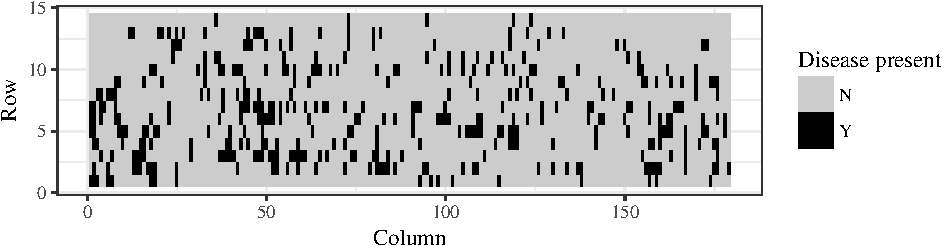
\includegraphics{supplement_files/figure-latex/endive-data-plot-1.pdf}
\caption{\label{fig:endive-data-plot}The endive dataset, a 14 \(\times\) 179 rectangular lattice with binary data encoding the incidence of footrot in endive plants.}
\end{figure}
Figure \ref{fig:endive-data-plot} shows a spatial dataset from Besag (\protect\hyperlink{ref-besag1977some}{1977}) consisting of binary observations located on a \(14 \times 179\) grid, indicating the presence (1) or absence (0) of footrot in endive plants. Here we consider fitting three models of increasing complexity to these data via pseudo-likelihood (Besag \protect\hyperlink{ref-besag1975statistical}{1975}) and apply simulation to obtain reference distributions for statistics based on the resulting estimators. This represents a parametric bootstrap approximation for sampling distributions, where simulation speed is important in rendering a large number of spatial data sets from differing models. For the spatial binary data, three centered autologistic models are considered as: (a) isotropic (Besag \protect\hyperlink{ref-besag1977some}{1977}; Caragea and Kaiser \protect\hyperlink{ref-caragea2009autologistic}{2009}), (b) ansiotropic with two dependence parameters, or (c) as in (b) but with large scale structure determined by regression on the horizontal coordinate \(u_i\) of each spatial location \(\boldsymbol s_i=(u_i,v_i)\). For each model, a four-nearest neighborhood is used (with natural adjustments for border observations) and the resulting conditional mass function has the form
\[
f_i(y(\boldsymbol s_i)| \boldsymbol y(\mathcal{N}_i), \boldsymbol \theta) =\frac{\exp[y(\boldsymbol s_i) A_i\{\boldsymbol y(\mathcal{N}_i)\}]}{ 1 +\exp[y(\boldsymbol s_i) A_i\{\boldsymbol y(\mathcal{N}_i)\}}, \quad y(\boldsymbol s_i)=0,1,
\]
from (1)-(2) with natural parameter functions,
\(A_i\{\boldsymbol y(\mathcal{N}_i)\} \equiv A_i\{\boldsymbol y(\mathcal{N}_i)\}(\boldsymbol \theta)\) given in Table \ref{tab:natural-params} here, that involve a vector \(\boldsymbol \theta\) of parameters contained in a model. In particular, \(\boldsymbol \theta\) denotes the collection of parameters \((\kappa, \eta)\) for Model (a), \((\kappa, \eta_u, \eta_v)\) for Model (b), and \((\beta_0,\beta_1, \eta_u, \eta_v)\) for Model (c).
\begin{table}[t]
\caption{Full conditional distributions (centered autologistic) of three binary MRF models.}
\label{tab:natural-params}
\centering
\begin{tabular}{|p{.1in}  p{6.0in} |}
\hline
(a)& Isotropic with $A_i\{\boldsymbol y(\mathcal{N}_i)\} = \log\left(\frac{\kappa}{1-\kappa}\right) + \eta\sum\limits_{\boldsymbol s_j \in \mathcal{N}_i}\{y(\boldsymbol s_j) - \kappa\}$, $\kappa\in(0,1)$, $\eta\in\mathbb{R}$, \& $\mathcal{N}_i =\{\boldsymbol s_i\pm (1,0),\boldsymbol s_i\pm (0,1)\}$     \\[.3cm]
(b) &Ansiotropic with $A_i\{\boldsymbol y(\mathcal{N}_i)\} = \log\left(\frac{\kappa}{1-\kappa}\right) + \eta_u\sum\limits_{\boldsymbol s_j \in N_{u,i}}\{y(\boldsymbol s_j) - \kappa\} + \eta_v\sum\limits_{\boldsymbol s_j \in N_{v,i}}\{y(\boldsymbol s_j) - \kappa\}$, $\kappa \in (0,1)$, horizontal/vertical dependence $\eta_u,\eta_v\in\mathbb{R}$, \& neighbors $\mathcal{N}_{u,i}=\{\boldsymbol s_i \pm (1,0)\}$, $\mathcal{N}_{v,i}=\{\boldsymbol s_i \pm (0,1)\}$   \\[.3cm]
(c) & like (b) with $A_i\{\boldsymbol y(\mathcal{N}_i)\}  = \log\left(\frac{\kappa_i}{1-\kappa_i}\right) + \eta_u\sum\limits_{\boldsymbol s_j \in N_{u,i}}\{y(\boldsymbol s_j) - \kappa_i\} + \eta_v\sum\limits_{\boldsymbol s_j \in N_{v,i}}\{y(\boldsymbol s_j) - \kappa_i\}$
but with $\kappa_i$ determined by  logistic regression $\mathrm{logit}(\kappa_i)  = \beta_0 + \beta_1 u_i$
on  horizontal coordinate $u_i$ of location $\boldsymbol s_i=(u_i,v_i)$,  \& $\beta_0,\beta_1\in\mathbb{R}$    \\
\hline
\end{tabular}
\end{table}
\begin{table}[ht]
\centering
\begin{tabular}{|l|rr|rrr|rrrr|}
  \hline &\multicolumn{2}{|c|}{Model (a)} & \multicolumn{3}{|c|}{Model (b)} & \multicolumn{4}{|c|}{Model (c)} \\
 \hline
 & $\eta$ & $\kappa$ & $\eta_u$ & $\eta_v$ & $\kappa$1 & $\eta_u$1 & $\eta_v$1 & $\beta_0$ & $\beta_1$ \\ 
  \hline
2.5\% & 0.628 & 0.107 & 0.691 & 0.378 & 0.106 & -0.225 & -0.221 & -1.822 & -0.003 \\ 
  50\% & 0.816 & 0.126 & 0.958 & 0.660 & 0.125 & 0.000 & 0.004 & -1.600 & -0.001 \\ 
  97.5\% & 1.001 & 0.145 & 1.220 & 0.921 & 0.145 & 0.209 & 0.214 & -1.391 & 0.001 \\ 
   \hline
\end{tabular}
\caption{Bootstrap percentile confidence intervals in all three autologistic models.} 
\label{tab:endive-table}
\end{table}
\begin{figure}
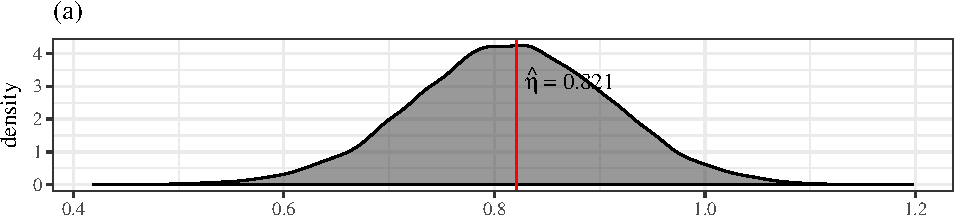
\includegraphics[width=1\linewidth]{supplement_files/figure-latex/endive-param-plot-1} 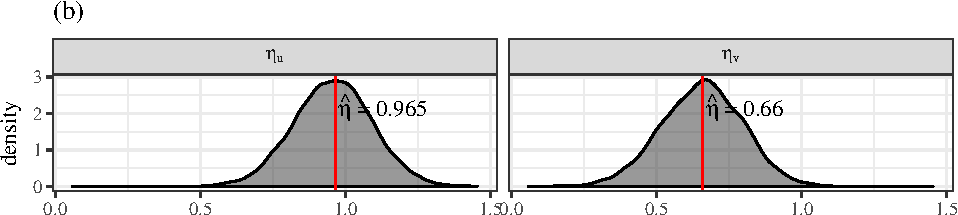
\includegraphics[width=1\linewidth]{supplement_files/figure-latex/endive-param-plot-2} 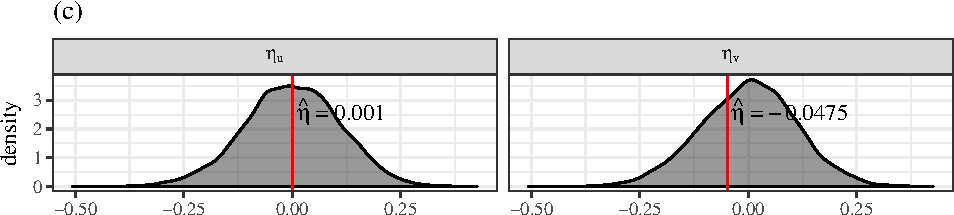
\includegraphics[width=1\linewidth]{supplement_files/figure-latex/endive-param-plot-3} \caption{Approximated sampling distributions of dependence parameter estimates  for the three centered autologistic models with four-nearest neighbors: (a)  isotropic  with one dependence parameter $\eta$, (b) ansiotropic with two dependence parameters $\eta_u$,  $\eta_v$, and (c) as in (b) but with a marginal mean involving regression on horizontal location $u_i$.}\label{fig:endive-param-plot}
\end{figure}
To calibrate confidence intervals for a model based on pseudo-likelihood estimates \(\widehat{\boldsymbol \theta}\), normal approximations are difficult as standard errors from pseudo-likelihood depend intricately on the spatial dependence, with no tractable form (cf.~Guyon \protect\hyperlink{ref-guyon1982parameter}{1982}). Instead, simulation with a model-based bootstrap may be applied to approximate the sampling distribution of \(\widehat{\boldsymbol \theta}\) under each model. Using conditional distributions prescribed by estimates \(\widehat{\boldsymbol \theta}\) as a proxy for the unknown parameters \(\boldsymbol \theta\), we generated \(10,000\) spatial samples of same size as the endive data from each binary MRF model based on the CGS or conclique-based Gibbs sampler (after a burn-in of \(1,000\) and thinning by a factor of \(5\) as conservative selections from trace plots). A bootstrap parameter estimate, say \(\widehat{\boldsymbol \theta}^*\), was obtained from each simulated sample. Relying on the applicability of a percentile parametric bootstrap approach (Davison, Hinkley, and others \protect\hyperlink{ref-davison1997bootstrap}{1997}, ch.~5), quantiles of the empirical distribution of bootstrap estimates are used to approximate quantiles of the sampling distribution of \(\widehat{\boldsymbol \theta}\). Figure \ref{fig:endive-param-plot} here displays the approximated distributions for dependence parameter estimates (e.g., \(\eta\), \(\eta_u\), \(\eta_v\)) in the three models, while Table \ref{tab:endive-table} here shows 95\% bootstrap confidence intervals for all model parameters. The intervals suggest that spatial dependence is a significant aspect of Models (a) and (b), but that most of the explanatory power of Model (c) lies in the model's large scale structure.

Using the same MRF-based simulations, we may also further assess the goodness-of-fit of all three models to the endive data through test statistics from {[}KLN{]}. That is, rather than the large-sample theory in {[}KLN{]}, we may more easily approximate reference distributions for such test statistics by evaluating these from the same collection of bootstrap simulated data sets. The subsequent p-values on model adequacy are \(0.04\), \(0.88\), and \(0.36\) for Models (a)-(c), respectively. These results support a conclusion of Besag (\protect\hyperlink{ref-besag2001markov}{2001}) regarding the lack-of-fit of Model (a) (i.e., isotropic autologistic model), but we find Models (b) and (c) are more compatible with these data by adding directional model structure, i.e., Model (b) as directional spatial dependence and Model (c) as a large-scale model component.

As suggested in this example, repeated simulation from MRF models can be useful for quantifying uncertainty in model fitting, provided that adequate data generation can be performed with reasonable speed. With the proposed CGS, the generation of the data sets for bootstrap reference distributions above required \(12.1\),
\(13.43\), and \(12.86\) seconds, respectively, for Models (a)-(c). In comparison, for the same number of data generations, the standard sequential Gibbs approach would take approximately \(25.9\) minutes for Model (a) and about \(26.8\) minutes for Models (b)-(c), and the numerical results here would be virtually identical to the CGS. Hence, the conclique-based sampler, while more efficient here in computational time, does not mix any faster than the standard Gibbs approach (i.e., exhibit better chain convergence). This aspect is examined in the simulation studies of Section 4 in greater detail.

\begin{mybibliography}{a}

\item
\hypertarget{ref-AL2006}{}
Athreya, K.B. and Lahiri, S.N. (2006). 
\emph{Measure theory and probability theory.} Springer, New York.

\item\hypertarget{ref-besag1975statistical}{}%
Besag, Julian. 1975. ``Statistical Analysis of Non-Lattice Data.'' \emph{The Statistician}, 179--95.

\item\hypertarget{ref-besag1977some}{}%
---------. 1977. ``Some Methods of Statistical Analysis for Spatial Data.'' \emph{Bulletin of the International Statistical Institute} 47 (2): 77--92.

\item\hypertarget{ref-besag2001markov}{}%
---------. 2001. ``Markov Chain Monte Carlo for Statistical Inference.'' \emph{Center for Statistics and the Social Sciences} 9: 24--25.

\item\hypertarget{ref-caragea2009autologistic}{}%
Caragea, Petruţa C, and Mark S Kaiser. 2009. ``Autologistic Models with Interpretable Parameters.'' \emph{Journal of Agricultural, Biological, and Environmental Statistics} 14 (3): 281.

\item \hypertarget{ref-cressie1993statistics}{}
Cressie, N. (1993). \emph{Statistics for spatial data}. Wiley, New York.


\item\hypertarget{ref-davison1997bootstrap}{}%
Davison, Anthony Christopher, David Victor Hinkley, and others. 1997. \emph{Bootstrap Methods and Their Application}. Vol. 1. Cambridge university press.

\item\hypertarget{ref-guyon1982parameter}{}%
Guyon, Xavier. 1982. ``Parameter Estimation for a Stationary Process on a d-Dimensional Lattice.'' \emph{Biometrika}, 95--105.

\item \hypertarget{ref-johnson2006}{}
Johnson, A.A.  (2009).   Geometric ergodicity of Gibbs samplers.  Dissertation, University of Minnesota. 
 

\item \hypertarget{ref-johnson2015geometric}{}
Johnson, A.A., and Burbank, O. (2015). Geometric ergodicity and
scanning strategies for two-component Gibbs samplers. 
\emph{Communications in Statistics - Theory and Methods}, \textbf{44},  
3125-3145.

\item \hypertarget{ref-kaiser1997modeling}{}%
Kaiser, Mark S, and Noel Cressie. 1997. ``Modeling Poisson Variables with Positive Spatial Dependence.'' \emph{Statistics \& Probability Letters} 35 (4): 423--32.


\item \hypertarget{ref-lee2001multiway}{}
Lee, J., Kaiser, M.S. and Cressie, N. (2001). Multiway
dependence in exponential family conditional distributions. 
\emph{Journal of Multivariate Analysis}, \textbf{79}   171-190.
 
\end{mybibliography}
\end{document}

 